在人类活动主导下的人-水关系中,根据我们的定义,人类社会的“水治理”深入影响了自然,
制定一个全面和直接的方法来确定水治理机制。

\subsection{人类主导时期的水资源治理分析框架}

水治理是指影响水的使用和管理的政治、社会、经济和行政系统,本质上是关于“谁获得水,何时获得水,如何获得水”。
因此,联合国开发计划署(UNDP)提出,由水治理相应地决定用水的三个核心方面:“什么时候用、用什么水?”“(重音),‘水如何为人类福祉提供不同的服务?“(目的)”和“谁能平等有效地使用水?””(分配)
\cite{undpwatergovernancefacility2016}。
首先,水资源压力不仅取决于气候(在许多地区日益稀缺和不确定性),还取决于灌溉和工业等经济活动日益无法满足的需求;蓄水可以解决部分问题,但不能解决全部问题
\cite{qin2019,wada2014,huang2021}。
其次,水如何服务于人类福祉的目的是考虑消费用途(例如,饮用和食品生产)和非消费用途(例如,能源生产)之间的权衡。
\cite{liu2017,florke2018,jaeger2019}。
第三,整个流域的水资源分配不仅取决于区域的社会经济和环境背景,还受到系统监管的影响
\cite{schmandt2021,speed2013}。
由于向人类主导体制的过渡导致了三个相互关联方面(压力、目的和分配)的实质性变化,单独考虑它们会导致水治理的系统性失败。

要理解水治理的成功与失败,关键的第一步是确定支撑水治理的不同制度。
水治理机制产生于相互关联的人-水系统(基于管理、制度和开发),以在社会-生态结构和功能中创造局部平衡
\cite{falkenmark2021,bressers2013,loch2020}。
例如,在人类主导的制度下,水库的灵活性使水资源压力更容易缓解;不断增长的能源和工业需求使供水服务向非供应部门倾斜;输水系统使水分配更有计划性(图~\ref{ch4:fig:framework}~A)
然而,缺乏一种全面而直接的方法来确定水治理制度的变化,这对加强水资源利用可持续性的努力构成了挑战。
填补这一空白是本文的目的,这对于人类和水系统的适当调整至关重要。

% 这里我们整合了三个方向,提出了描绘流域人水关系的指数
在这里,我们用相应的指标(见方法)描述了水治理的三个方面(压力、目的和分配),从而通过对它们进行同等加权,得出了综合水治理指数(IWGI),以表明水治理的结果(见图\ref{ch4:fig:framework}~B)。
% 使用案例研究
然后,通过将该指数应用于一个典型的快速变化的大流域(YRB),我们展示了IWGI如何帮助全面而直接地检测和描述复杂的水治理机制。
在综合分析了水的需求、供应、经济结果和制度的变化之后,我们解释了政权转变的主要原因。
% 最后总结出一般性框架
最后,我们提出了一个普遍的政权过渡模式,为探索大流域治理面临的挑战提供了一个协调方法的实践指南。


首先,本章研究从压力(Stress)、目的(Purpose)和分配(Allocation)三个方面构建了综合水治理指数(Integrated Water Governance Index, IWGI),见图~\ref{ch4:fig:framework}。
然后,本章研究利用变化点检测方法分析了$1965\sim2013$年IWGI的变化。
每个维度的指标经标准化后,分析其对IWGI趋势变化的影响和贡献。


\begin{figure}[!ht]
\centering
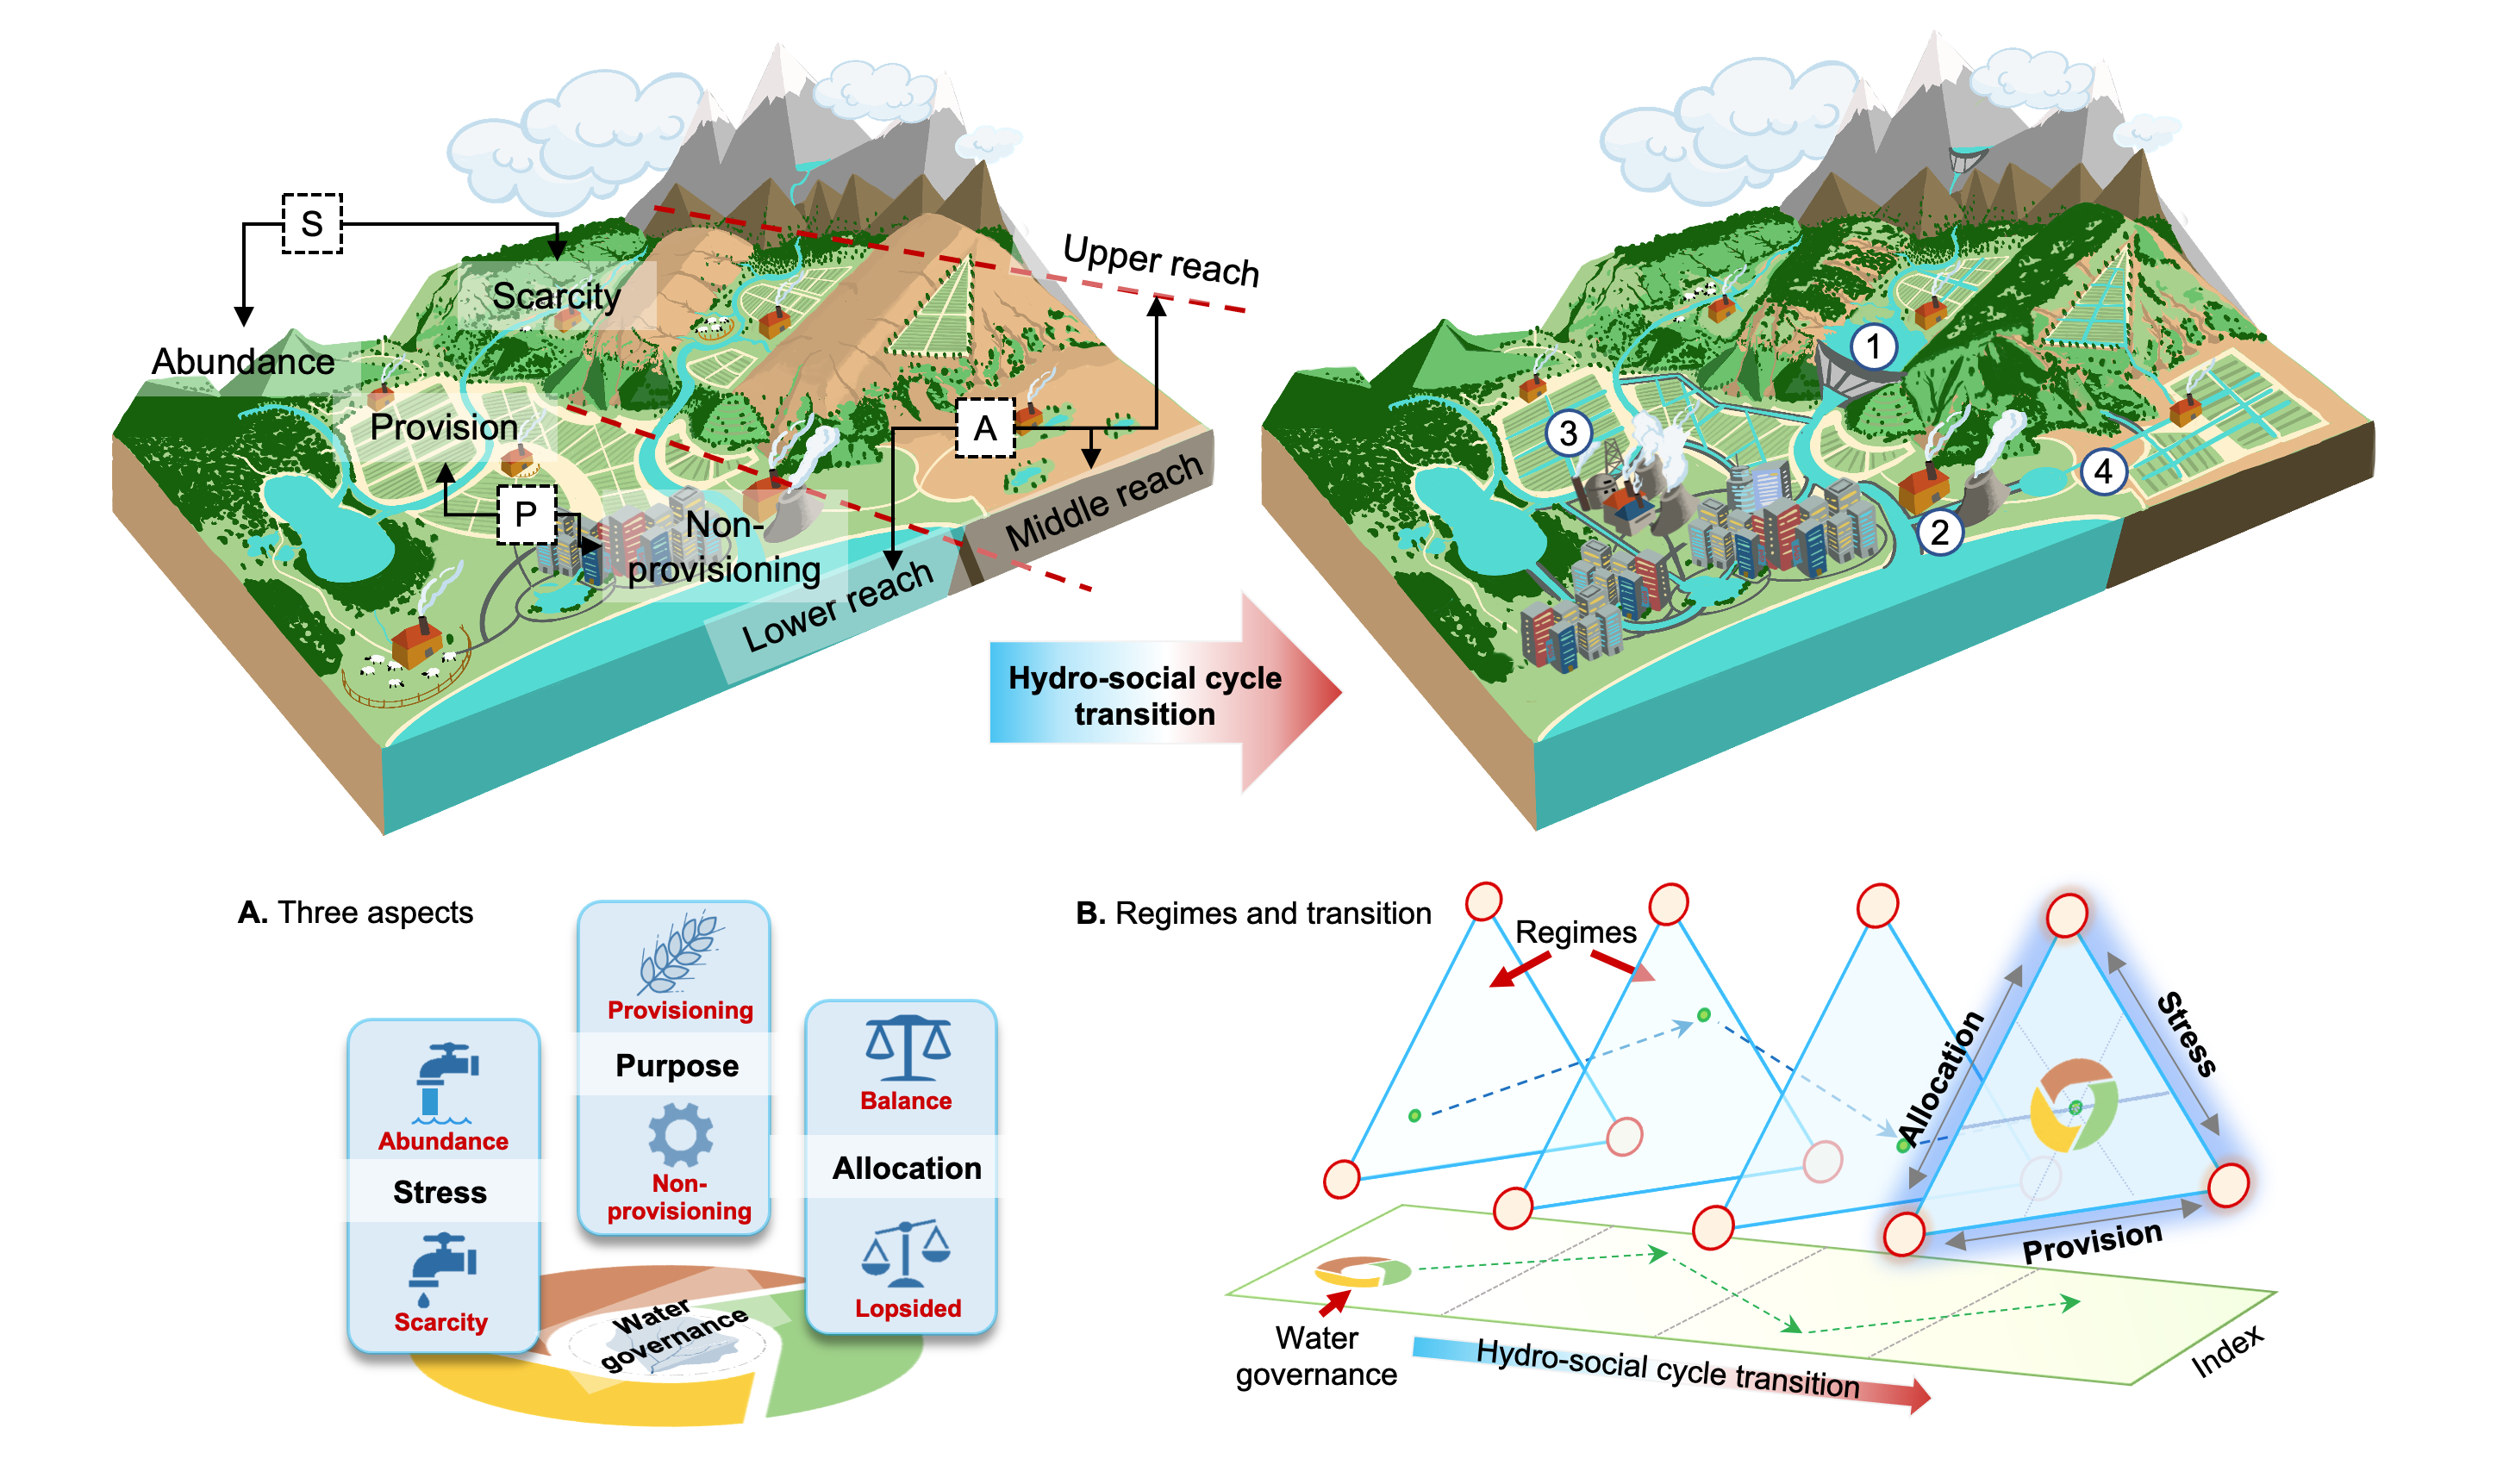
\includegraphics[width=\textwidth]{img/ch4/framework.png}
\caption[利用综合水治理指数(IWGI)识别水社会循环转型中的水治理机制]{
    利用综合水治理指数(IWGI)识别水社会循环转型中的水治理机制。水资源压力(S)、供水服务的目的(P)和水资源分配(A)是需要考虑的三个方面(\textbf{A.})。随着水系社会循环的转变,以人为主导的制度影响着水治理的这些方面。例如,水库的建设(1)旨在缓解水资源紧张;能源和工业增长(2);水铅密集型农业(3);输水系统(4)控制水的分配。因此,该方法是结合三个方面的相应指标,然后IWGI的突变可以表明水治理的政权转移(\textbf{B.})。
}
\label{ch4:fig:framework}
\end{figure}

\subsection{研究区域定义}
\label{ch4:sec:region}

本章研究将黄河流域划分为四个区域,以计算考虑社会经济和自然条件的指标。该划分与出版物和YRCC \cite{shuilibuhuangheshuiliweiyuanhui,wang2019c,wang2016e}的习惯模式一致,因此可以区分四个重要的水文站(见图~\ref{fig:YRB})。
\begin{itemize}
\item \textbf{黄河源区(SR):}超过$50\%$的自然径流来自这个地区。这里人口稀少,经济不发达,最生态的功能是产水。
\item \textbf{黄河上游(SR):}这个地区人均灌溉土地面积最高,有大量的大型灌溉土地。然而,灌溉效率相对较下游低得多。
\item \textbf{黄河源区(MR):}黄河流经著名的富沙区黄土高原,这里是黄河淤积最多的地区,也是土壤侵蚀风险最高的地区。“退耕还林”工程显著改变了这里的水资源利用,扭转了这一局面。
\item \textbf{黄河下游(LR):}下游地区人口密集,传统农业发展轨迹,曾是最大的用水区。然而,随着产业转型的进行,农业的比重不断下降,但LR仍是各方面用水最多的地区。
\end{itemize}

% 补充图片1:研究区示意图
\begin{figure*}[hbtp!]
\centering
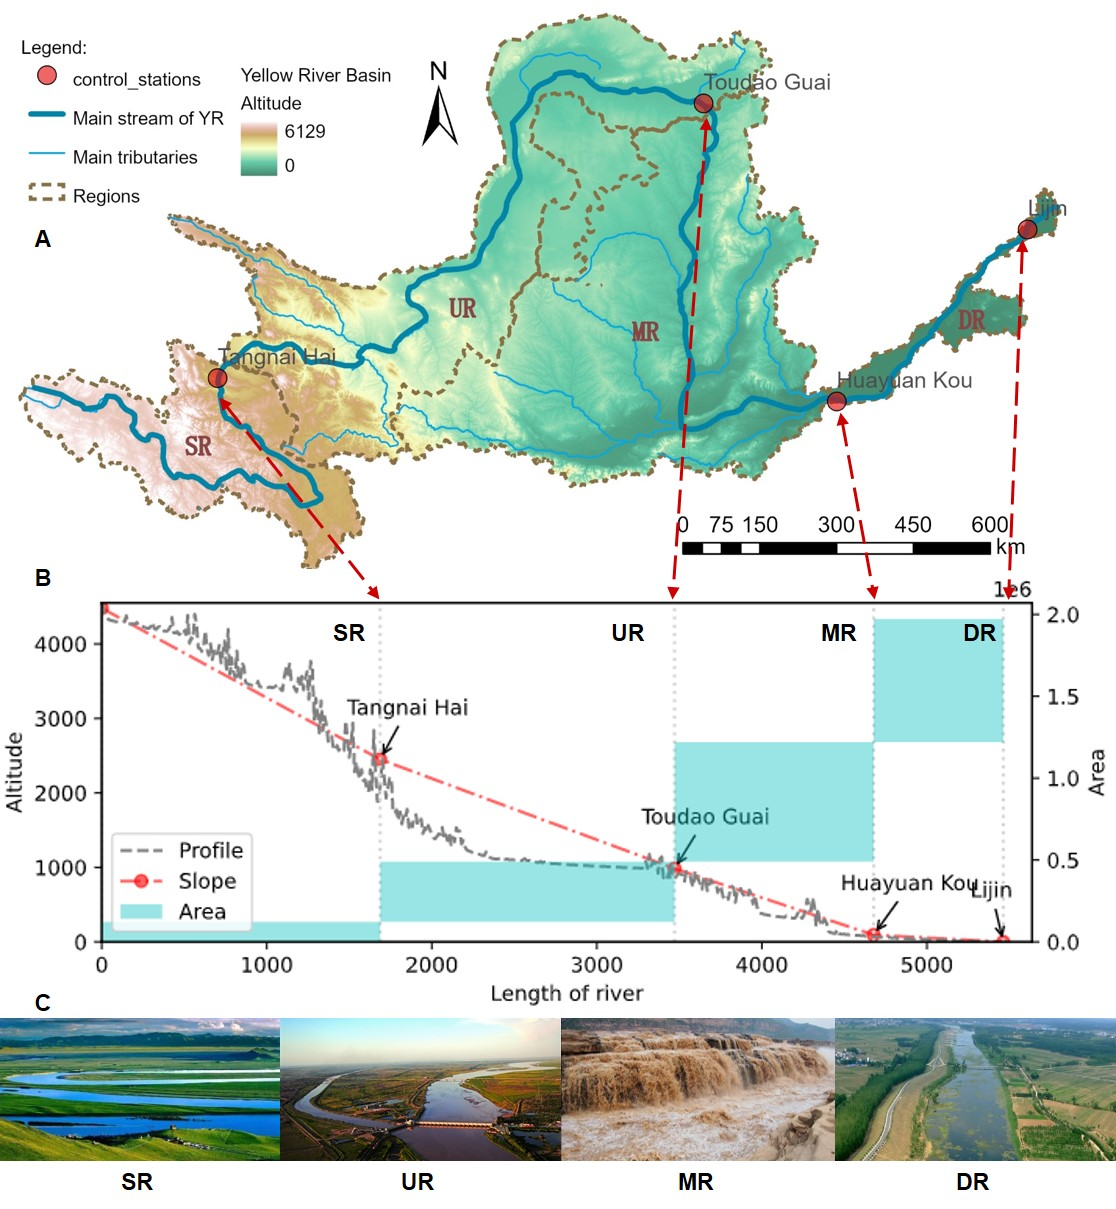
\includegraphics[width=\textwidth]{img/ch4/s1_study_area.jpg}
\caption[黄河流域子区域划分]{黄河流域子区域划分。
    \textbf{A.}黄河下游与盆地划分示意图(SR:源区,UR:上区,MR:中区,DR:下游区)
    \textbf{B.}黄河主河道剖面图。水文站控制SR、UR、MR和DR。
    \textbf{C.}黄河流域不同地区的典型景观。
}
\label{fig:YRB}
\end{figure*}


\subsection{水资源治理综合指数}

% 将三者合一起,即:
如框架图~\ref{ch4:fig:framework}所示,IWGI结合了水治理的三个方面(压力、目的和分配)。每个维度保持两个方向,本章研究假设水社会循环与其中一个方向对齐,分别为:

\begin{equation}
    Transformation \propto S*P*A
\end{equation}

本章研究选择了一个指标($I_x$, $x=S$, $P$,或$A$,分别对应压力,目的和分配)来有效地量化这些方面。然后将上式转化为自然对数,便于计算:

\begin{equation}
    Transformation \propto ln(I_S) + ln(I_P) + ln(I_A)
\end{equation}

那么,综合水治理指数(IWGI)是标准化指标$I'_x$的平均值:
\begin{equation}
    IWGI = (I'_S + I'_P + I'_A) / 3
\end{equation}

其中:
\begin{equation}
    I'_x = (I_x - I_{x, min}) / (I_{x, max} - I_{x, min})
\end{equation}

\subsubsection*{水资源压力指数}

本章研究采用Qin等人(2019)提出的稀缺性-韧性-可变性(SFV)水胁迫指数来评价水胁迫\cite{qin2019}。这一指标考虑了管理措施(如水库的建设)和用水结构变化对水资源短缺评估的影响。SFV指数考虑了水资源的灵活性和可变性,从发展的角度更关注水资源的动态响应,是衡量水资源压力\cite{qin2019}时间变化的有效指标。
根据黄河流域的水文和经济背景,划分了四个二级区域(源区、上区、中区和下区,见\textit{ Supporting  Information S1})。整个YRB的水分胁迫指标$I_S$为各区域sfv指数的平均值:

\begin{equation}
    I_S = \frac{1}{4} * \sum_{i=1}^4 SFV_{i}
\end{equation}

其中$SFV_i$为区域$i$的SFV指数$SFV_i$,结合了以下三个指标:

首先,对于稀缺性,$A_{i, j}$为区域$i$在第$j$年的耗水量占多年平均径流量的比例(本研将为黄河流域划分为四个子区域,见\ref{ch4:sec:region}\nameref{ch4:sec:region}):

\begin{equation}
    A_{i, j} = \frac{WU_{i,j}}{R_{i, avg}}
\end{equation}

其次,对于灵活性,$B_{i, j}$是第$i$年和第$j$地区的不灵活用水$WU_{inflexible}$(例如能源行业冷却用水或人类和牲畜)占平均多年径流量的比例:

\begin{equation}
    B_{i, j} = \frac{WU_{i, j, inflexible}}{R_{i, avg}}
\end{equation}

最后,易变性(Variability)还考虑了水库容量和蓄水对自然径流波动的积极影响:
\begin{gather}
    C_i = C1_i * (1 - C2_i) \\
    C1_{i, j} = \frac{R_{i, std}}{R_{i, avg}} \\
    C2_{i} = \frac{RC_{i}}{R_{i, avg}}, \ if RC < R_{i, avg} \\
    C2_{i} = 1, \ if RC >= R_{i, avg}
\end{gather}

上式中,$R_{i, avg}$为$i$区域的平均径流量,$RC_i$为$i$区域水库的总库容,$R_{i, std}$为$i$区域径流量的标准差。

最后,假设三个指标(稀缺性、灵活性和可变性)具有相同的权重,我们可以将它们归一化后计算出$SFV$指标:

\begin{gather}
    V = \frac{A_{normalize} + B_{normalize} + C_{normalize}}{3}\\
    a = \frac{1}{V_{max} - V_{min}};\\
    b = \frac{1}{V_{min} - V_{max}} * V_{min}\\
    SFV = a * V + b
\end{gather}


\subsubsection*{水资源供给指标}

为了量化目的$I_P$,本章研究使用了用水的非供应目的份额(NPS)作为指标。供应目的用水($WU_{pro}$)包括家庭用水、灌溉用水和牲畜用水,非供应目的用水($WU_{non-pro}$)包括工业用水和城市服务用水。本章研究计算NPS为:

\begin{equation}
    NPS = \frac{WU_{pro}}{WU_{pro} + WU_{non-pro}}
\end{equation}

在本研究中,本章研究将牲畜用水、城乡生活用水和农业用水作为供应用水,因为它们直接服务于生存。其他的是非供应:服务和工业用水,因为它们主要为经济服务。

\subsubsection*{水资源分配指标}
为了描述分配$I_A$,本章研究设计了一个基于熵的分配度量指标,它衡量水分配的均匀程度:

\begin{equation}
    I_A = CEM = \sum_{i=1}^N -log(p_{i}) * p_{i}
\end{equation}

其中$p_{i}$为区域$i$与整个流域的水量比例(这里,$N=4$考虑了黄河流域的划分区域,见\textit{ Supporting  Information S1})。

\subsection{变化点检测}

本章研究采用Pettitt(1979)提出的的变化点检测方法,在不假设数据分布的情况下,对连续数据的水文时间序列中的单个变化点进行检测\cite{pettitt1979}。
它测试的原假设$H0$是:独立同分布的变量不存在存在变化趋势差异,备择假设则为存在一个变化趋势点。
数学上,将随机变量序列分为$\mathrm{x}_{1}, \mathrm{x}_{1}, \ldots, x_{t_{0}}$和$x_{t_{0}+1}, x_{t_{0}+2}, \ldots, x_{T}$表示的两段,如果每段都有一个共同的分布函数,即$F_1(x)$、$F_2(x)$和$F_1(x) \neq F_2(x)$,则在$t_0$处确定变化点。为实现变化点的识别,定义统计指标$U_{t,T}$如下:

\begin{equation}
    U_{t, T} = \sum_{i=1}^t\sum_{j=t+1}^T sgn(X_i - X_j), 1 \leq t < T
\end{equation}

其中:
\begin{equation}
    \operatorname{sgn}(\theta)= \begin{cases}1 & \text { if } \theta>0 \\ 0 & \text { if } \theta=0 \\ -1 & \text { if } \theta<0\end{cases}
\end{equation}

找到最可能的变化点$\tau$,其值满足$K_{\tau} = max|U_{t, T}|$,与值$K_{\tau}$相关的显著性概率近似计算为:

\begin{equation}
    p=2 \exp \left(\frac{-6 K_{\tau}^{2}}{T^{2}+T^{3}}\right)
\end{equation}
给定某个显著性水平$\alpha$,如果$p < \alpha$,本章研究拒绝原假设,并得出结论,$x_{\tau}$是水平$\alpha$的显著变点。

本章研究使用$\alpha = 0.001$作为p值的阈值水平,这意味着统计上显著的变化点判断有效的概率大于$99.9\%$。本章研究将该序列分为两个,并分别分析每个序列,直到检测到所有重要的变化点。虽然在$\alpha = 0.001$的正文中有两个断点,但是从$0.0005$到$0.05$的阈值并不影响本章研究的结果,并且本章研究识别的断点是鲁棒的(参见图~S3)。

\subsection{数据来源与处理}
为了计算 IWGI ,本章研究需要计算多个指标及子指标,所有使用的数据集都在表\ref{ch4:tab:data_source}中列出。

% Table generated by Excel2LaTeX from sheet '数据集'
\begin{table}[htbp]
    \centering
    \caption{数据分类与来源}
      \begin{tabularx}{\textwidth}{LLLLL}
      \toprule
      数据集   & 数据类型  & 空间尺度  & 时间尺度  & 数据来源 \\
      \midrule
      行政区水资源利用 & 统计    & 市级行政单元 & $1965-2013$ & Zhou等人2020 \\
      子流域水资源使用 & 统计    & 二级子流域 & $2003-2019$ & 水资源公报 \\
      GDP数据 & 统计    & 省级行政单元 & $1949-2019$ & 万德数据库 \\
      水库数据集 & 水文    & 站点数据  & $1949-2015$ & Wang等人2019 \\
      实测泾流量 & 水文    & 站点数据  & $1949-2019$ & Wang等人2019 \\
      黄河流域相关法律 & 文献    & 流域相关文件 & $1949-2013$ & 黄河流域规划 \\
      黄河水利委员会历史 & 文献    & 流域相关文件 & $1949-2002$ & 黄河水利委员会档案馆 \\
      黄河大事件 & 文献    & 流域相关文件 & $1949-2015$ & 黄河水利委员会档案馆 \\
      \bottomrule
      \end{tabularx}%
    \label{ch4:tab:data_source}%
\end{table}%
  

我们使用GDP数据;水资源数据来源于第二次国家水资源评估方案\cite{zhou2020}和统计年鉴\url{http://www.yrcc.gov.cn/other/hhgb/}。
水资源利用数据集由Zhou et al. \cite{zhou2020}发布,该数据集记录了不同部门的水资源利用情况以及地级的社会经济状况。第二次国家水资源评价计划主要提取了2002年国家发展和改革委员会、水利部牵头启动的该数据集(详见ref(1)和\url{http://www.mwr.gov.cn/english/publs/})。从那时起,使用相同标准的调查统计数据与2013年的行政区划进行了补充和协调。

数据涵盖了用水的四个大类下的子类别:农业(IRR)、工业(IND)、城市(URB)和农村(RUR)用水(详见Zhou et al., \cite{zhou2020})。
每个分类用水部门在县尺度上都存在不确定性,但由于校正数据是使用水平衡方法进行统计信息,因此该数据足以用于本研究中使用的区域尺度。

\subsubsection{水资源数据集}
储层数据集由Wang et al. \cite{wang2019c}收集,其中介绍了1949年以来在黄河上游新建的重要储层(图~\ref{fig:reservoirs})。YRCC在其中标注了调控型储层,见\url{http://www.yrcc.gov.cn/hhyl/sngc/})。此外,从水文站测量得来的年径流数据与\cite{wang2019c}和\cite{wang2016e}使用的数据集相同。

\begin{figure}[tb]
    \centering
    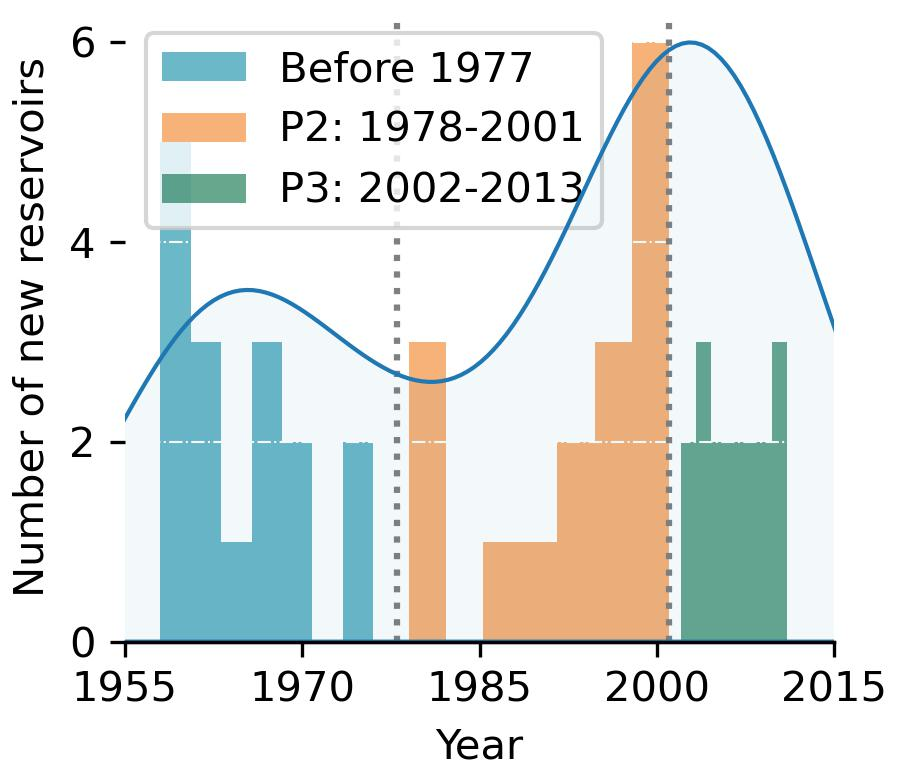
\includegraphics[width=0.6\linewidth]{img/ch4/reservoirs.jpg}
    \caption{
        各年新增水库数量.
    }
    \label{fig:reservoirs}
\end{figure}

\subsubsection{政治数据集}

政策数据集收集了\cite{shuilibuhuangheshuiliweiyuanhui}书中所列的黄河流域相关法律政策,由流域级以上部门(如长江水利委)(如国家机关)颁布实施(表~\ref{ch4:tab:policies})。
此外,有些很难分类;黄河水利委员会的黄河大事件记录了黄河流域的许多治理实践,但这并不是一个里程碑;我们从\url{http://www.yrcc.gov.cn/hhyl/hhjs/}中收集它们。

% Table generated by Excel2LaTeX from sheet '黄河流域法律政策'
\begin{table}[htbp]
    \centering
    \caption{黄河流域法律政策}
      \begin{tabularx}{\textwidth}{L p{1.5cm} L}
      \toprule
      法律或政策名称 & \multicolumn{1}{l}{施行或修订时间} & 颁布机构 \\
      \midrule
      中华人民共和国水法 & 1,988 & 全国人民代表大会常务委员会 \\
      中华人民共和国水法  修正 & 2,002 & 全国人民代表大会常务委员会 \\
      中华人民共和国水法  第一次修订 & 2,009 & 全国人民代表大会常务委员会 \\
      中华人民共和国水法  第二次修订 & 2,016 & 全国人民代表大会常务委员会 \\
      中华人民共和国水污染防治法 & 1,984 & 全国人民代表大会常务委员会 \\
      中华人民共和国水污染防治法  修正 & 1,996 & 全国人民代表大会常务委员会 \\
      中华人民共和国水污染防治法  第一次修订 & 2,008 & 全国人民代表大会常务委员会 \\
      中华人民共和国水污染防治法  第二次修订 & 2,018 & 全国人民代表大会常务委员会 \\
      取水许可和水资源费征收管理条例 & 2,006 & 中华人民共和国国务院 \\
      取水许可和水资源费征收管理条例  第一次修订 & 2,017 & 中华人民共和国国务院 \\
      黄河水量调度条例 & 2,006 & 中华人民共和国国务院 \\
      黄河可供水量分配方案 & 1,987 & 中华人民共和国国务院 \\
      取水许可管理办法 & 2,008 & 中华人民共和国水利部 \\
      取水许可管理办法  第一次修订 & 2,015 & 中华人民共和国水利部 \\
      取水许可管理办法  第二次修订 & 2,017 & 中华人民共和国水利部 \\
      黄河水量调度条例 & 2,006 & 中华人民共和国国务院 \\
      黄河可供水量年度分配及干流水量调度方案 & 1,998 & 国家发展计划委员会,水利部 \\
      黄河水量调度管理办法 & 1,998 & 国家发展计划委员会,水利部 \\
      黄河水权转换管理实施办法 & 2,004 & 水利部 \\
      取水许可和水资源费征收管理条例 & 2,006 & 中华人民共和国国务院 \\
      取水许可证制度实施办法 & 1,993 & 中华人民共和国国务院 \\
      建设项目水资源论证管理办法 & 2,002 & 国家发展计划委员会,水利部 \\
      水利工程管理体制改革实施意见 & 2,006 & 中华人民共和国国务院 \\
      \bottomrule
      \end{tabularx}%
    \label{ch4:tab:policies}%
  \end{table}%
  
